\documentclass[12pt, a4paper]{article}

% Packages{{{
\usepackage[sc]{mathpazo}
\usepackage{graphicx}
  \graphicspath{ {./images/} }
\usepackage[T1]{fontenc}
  \linespread{1.2}
\usepackage{microtype}
\usepackage{soul}
\usepackage{xcolor}

\usepackage[english]{babel}

\usepackage[margin=20mm,columnsep=25pt]{geometry}
\usepackage[hang, small,labelfont=bf,up,textfont=it,up]{caption}
\usepackage{booktabs}

\usepackage{lettrine}

\usepackage{enumitem}
  \setlist[itemize]{noitemsep}
  % \setlist[enumerate]{noitemsep}

\usepackage{titlesec}
% \renewcommand\thesection{Roman{section}}
% \renewcommand\thesubsection{{subsection}}
% \titleformat{\section}[block]{\Large\scshape\centering}{\thesection.}{0.5em}{}
\titleformat{\section}[block]{\Large\scshape\centering}{}{0em}{}
% \titleformat{\subsection}[block]{\large}{\thesubsection.}{1em}{\textbf}
\titleformat{\subsection}[block]{\large}{}{0em}{\textbf}
\titleformat{\subsubsection}[block]{}{}{0em}{\textbf}

% \usepackage{fancyhdr} % Headers and footers
% \pagestyle{fancy} % All pages have headers and footers
% \fancyhead{} % Blank out the default header
% \fancyfoot{} % Blank out the default footer
% \renewcommand{\headrulewidth}{0pt}
% \fancyhead[RE,LO]{\thepage} % Custom footer text

\usepackage{titling}
\usepackage{fancyhdr}                                       % Fancy Header and footer
\usepackage{hyperref}
%}}}


% Title{{{
\setlength{\droptitle}{-4\baselineskip}

\pretitle{\begin{center}\Huge\bfseries}
\posttitle{\end{center}}
\title{Management Information System}
\author{ by
  \textsc{Swapnil}%\\[1px]
}
\date{}
%}}}

\begin{document}
% FontMatter {{{
% \begin{titlingpage}
  \maketitle
  % \thispagestyle{empty}
  % \setcounter{tocdepth}{3}
  % \tableofcontents
% \end{titlingpage} }}}

\section{Influence of Mordern Business on Information System}%{{{
\lettrine[nindent=0em,lines=2]{W}ith constant change and evolution of customer
preferences and requirements, businesses need to bring out new methods and
innovative techniques to survive the market and continue to function as per
the customer demands.

Implementation of an Information System in such cases could help in
controlling the internal and external processes.

Benefits of Information System are as follows:

\subsection{New Products and Services}
Businesses need a well organized \emph{business information system}.
It \hl{helps in analyzing independent processes and enables organized work
activities}. Also allows companies to understand how to develop, sell
services or products.

\subsection{Information Storage}
This helps in keep logs of different `important' activities so, in case of
a problem, people can make better decisions. \hl{Business information
system makes it easier to store operational data. revision histories,
different records and documents.} Generally, the information is stored in a
database which makes data retrieving and processing easier.

\subsection{Simplified Decision Making}
It \hl{simplifies the process of decision making and simplifies the process
of delivering the required information} which helps us to take better
decisions.

\subsection{Behavioral Change}
It is effective in implementing better communication between the employers and
the employees. Information systems store documents and files in a common
database which can be accessed and shared by the employees. It helps oversee
the flow of information between the management and the lower-level employees.
\hl{Allows the front-line employees to be a part of the decision making
process and hence feel motivated and committed towards doing a task.}

%}}}

% Diff tps and mis {{{
\begin{table}[ht]
  \centering
  \begin{tabular}{p{2cm}p{6cm}p{6cm}}
  \toprule
  &
  \textbf{TPS}&
  \textbf{MIS}\\
  \cmidrule(r){2-3}
 
  \emph{Input}&
  Transaction/events &
  Output from TPS\\
  \midrule

  \emph{Output}&
    Data entry, listing, sorting, merging and updating. &
    Routine reports, simple models, low level analysis.\\
  \midrule

  \emph{Users}&
    Operational personals, lower-level managers, supervisors. &
    Middle-level manager\\
  \midrule

  \emph{Goal}&
    Records and processes transactions. &
    Production of summary and exception reports.\\
  \midrule

  \emph{Decision \& support} &
    Provides decision support to lower-level managers &
    Provide decision supports to tactical-level managers\\
  \bottomrule

\end{tabular}
  \caption{Difference between Transaction Processing System and Management
  Information System.\label{difftpsmis}}
\end{table}%}}}

\section{Types of Information System}%{{{
\subsection{Transaction Processing System}%{{{
Transaction processing is a way of computing that divides work into
individual, indivisible operations, called transactions. A transaction
processing system is a software system, or software/hardware combination, that
supports transaction processing.%}}}

\subsection{Management Information System}%{{{
A management information system is an information system used for
decision-making, and for the coordination, control, analysis, and
visualization of information in an organization. The study of the management
information systems involves people, processes and technology in an
organizational context. In a corporate setting, the ultimate goal of using
management information system is to increase the value and profits of the
business.%}}}

\subsection{Decision Support System}%{{{
A decision support system (DSS) is an information system that supports
business or organizational decision-making activities. DSSs serve the 
management, operations and planning levels of an organization (usually
mid and higher management) and help people make decisions about
problems that may be rapidly changing and not easily specified in
advance -- IE unstructured and semi-structured decision problems.
Decision support systems can be either fully computerized or
human-powered, or a combination of both.

Some important characteristics of DSS are:
\begin{itemize}
  \item Adaptability and flexibility
  \item High level of interactivity
  \item Ease of use
  \item Efficiency and effectiveness
  \item Complete control by decision-makers
  \item Ease of development
\end{itemize}%}}}

\subsection{Expert System}%{{{
\hl{Expert system is a computer system emulating the decision-making ability
of a human expert}. \hl{These systems are designed to solve complex problems
by reasoning through bodies of knowledge}, represented mainly as if–then rules
rather than through conventional procedural code. Expert systems were among
the first truly successful forms of artificial intelligence software. An
expert system is divided into two subsystems: the inference engine and the
knowledge base. The knowledge base represents facts and rules. The inference
engine applies the rules to the known facts to deduce new facts. Inference
engines can also include explanation and debugging abilities%}}}
%}}}

\section{Application of databases in business}%{{{
\subsection{Customer Relationship Management}
\hl{CRM database can help small business manage its customers.} A CRM
database organizes all the information a company has about its accounts,
contacts, leads and opportunities.

\subsection{Inventory Tracking Database}
\hl{It helps a retail business manage how much inventory is in a
warehouse, in a storage room and on store shelves.}

\subsection{Payroll and Scheduling Database}
\hl{It simplifies scheduling and help prevent payroll errors.}

An employee database contains such fields as hourly wage, salary or 
commission, tax withholding rates, year-to-date income and accrued vacation
time.

\subsection{Business Data Analysis}
\hl{Databases make the process of analyzing data and predicting future trends
easier.}
%}}}

\section{E-commerce}%{{{
E-commerce is the activity of electronically buying or selling of products on
online services or over the Internet. E-commerce draws on technologies such as
mobile commerce, electronic funds transfer, supply chain management, Internet
marketing, online transaction processing, electronic data interchange,
inventory management systems, and automated data collection systems.
E-commerce is in turn driven by the technological advances of the
semiconductor industry, and is the largest sector of the electronics industry.
%}}}

\section{E-Business}%{{{
Any kind of business or commercial transaction that includes sharing
information across the internet. Commerce constitutes the exchange of products
and services between businesses, groups, and individuals and can be seen as
one of the essential activities of any business.
%}}}

% Diff between ecom and ebuis {{{
\begin{table}[ht]

  \caption{Difference between e-commerce and e-business}
\resizebox{\columnwidth}{!}{%
  \begin{tabular}{p{0.2cm}p{3cm}p{4cm}}
  \toprule
  &
  \textbf{E-commerce}&
 \textbf{E-business}\\
  \cmidrule(r){2-3}

  I &
    Refers to the performing of online commercial activities, transactions
    over internet. &
    Refers to the performing of all type of business activities through
    internet.\\
  \midrule

  II &
    It is a narrow concept and it is considered as a subset of e-business. &
    It is a broad concept and it is considered as a super-set of e-commerce\\
  \midrule

  III &
    Commercial transactions are carried out in e-commerce &
    Business transactions are carried out in e-business\\
  \midrule

  IV &
    Transactions are limited &
    Transactions are not limited \\
  \midrule

  V &
    It includes activities like buying and selling products, making monetary 
    transactions etc over the internet. &
    It includes activities like procurement of raw materials/goods, customer
    education, supply activities buying and selling product, making monetary
    transaction etc over internet. \\
  \midrule

  VI &
    Requires only the use of a website. &
    Requires use of multiple websites, CRMs, ERPs, that connect different
    business processes. \\
  \midrule
 
  VII &
    Involves mandatory use of internet. &
    Involves use of: Internet, Intranet, Extranet \\
  \bottomrule

\end{tabular}%
}
\end{table}
%}}}

\section{Categories of E-commerce}%{{{
\subsection{Business to Business}
Refers to all electronic transactions of goods and sales that are conducted
between two companies. This type of e-commerce typically \hl{explains the
relationship between the producers of a product and the wholesalers who
advertise the product for purchase to consumers}. Sometimes this allows
wholesalers to stay ahead of their competition.

\subsection{Business to Consumer}
\hl{The most common form of e-commerce, B2C e-commerce deals with
electronic business relationships between businesses and consumers.}

This e-commerce category also enables businesses to develop a more
personalized relationship with their customers.

\subsection{Consumer to Consumer}
\hl{This level of e-commerce encompasses all electronic transactions that take
place between consumers.}

Generally, these transactions are provided by online platforms (such as UPI),
but often are conducted through the use of social media networks (Facebook
marketplace) and websites (ebay).

\subsection{Consumer to Business}
\hl{Not the most traditional form of e-commerce, C2B e-commerce is when a
consumer makes their services or products available for companies to purchase.}

An example of this would be a graphic designer customizing a company logo or a
photographer taking photos for an e-commerce website. %}}}

\section{different IT tools used to grow business}
\subsection{IT applications used in business.}%{{{
There are 7 types of business technology tools to save time and money
\begin{enumerate}
  \item Task management tools.
  \item Email and social marketing.
  \item Social media scheduling tools.
  \item Scheduling meetings.
  \item Obtaining e-Signature.
  \item Finding and retaining business clients.
  \item Document collaboration.
\end{enumerate}%}}}

% diff bet inter and extranet{{{
\begin{table}[h]
 \caption{Difference between internet and extranet}
\resizebox{\columnwidth}{!}{%
\begin{tabular}{lp{3cm}p{3cm}}
  \toprule
  &
  \textbf{Internet}&
  \textbf{Extranet}\\
  \cmidrule(r){2-3}

  I &
    It is used as public network. &
    It is used as private network. \\
  \midrule

  II &
    Less secure &
    More secure\\
  \midrule

  III &
    Anyone can access it without a valid username or password &
    No one can access it without a valid username or password\\
  \midrule

  IV &
    Large number of users can access it &
    A limited number of users can access it\\
  \midrule

  V &
    It acts a tool for sharing information all over the world. &
    It acts as a medium for sharing information between the internal and
    external members.\\
  \midrule

  VI &
    Internet is not owned by anyone. &
    Extranet is owned by a single or multiple organization \\
  \midrule
 
  VII &
    Not managed by either authority. &
    Managed by numerous organizations.\\
  \bottomrule
\end{tabular}
}
\end{table}
%}}}

\section{Advantages of e-commerce}%{{{
Here are the advantages of e-commerce \footnote{As per 
\href{https://sell.amazon.in/seller-blog/advantages-of-ecommerce}{this amazon blog}}

\subsection{Faster buying process}
\hl{Customers can easily browse through many items at a time and buy what they
like.}

Customers can easily find items that are available in physical stores far away
from them or not found in their locality.

\subsection{Cost reduction}
\hl{Sellers can reduce how much is spent in store upkeep.}

An e-commerce store is affordable and requires less investment when compared
with a physical store. This is also a good opportunity for individual and
small scale sellers who want to earn an income but don’t have the required
start-up capital.

\subsection{Product and price comparison}
\hl{In e-commerce sellers as well as consumers can compare different products
as well as the price of those products, while in physical stores a person has
very little variety to compare those product to.}

It helps to save time when making this comparison, as all details are
available on the shopping site.

\subsection{Flexibility for customers}
Sellers can provide flexibility to customers. One highlight is that the
product and services are ready 24x7. The result is that seller can offer his
item any place, any time.

There are also reviews on the things to buy. This gets the buyers trusts in
different store based on the number of positive reviews.
Sellers can sell on an online marketplace confidently knowing that there are
plenty of buyers.

\subsection{No reach limitations}
With no limitations on how many people can view products on an e-commerce
site, a seller can invest more on higher quality products and attracts even
more customers.
Resulting in higher chances of that customer to actually buy those product.
%}}}

\section{Disadvantages of e-commerce}%{{{
\begin{itemize}
  \item As there is a requirement of the internet to use e-commerce, it is
    possible that the internet may be slow.
  \item It does not have any universal standard for reliability and quality.
  \item There can be compatibility issues.
  \item Security is another concern of using e-commerce.

    We have seen security breaches many times where the customer's information
    got stolen. Some of the big concerns with customers include identity
    theft, credit card theft, etc.

  \item E-commerce uses a public key that is not secure.

  \item It is a major drawback in E-commerce that there is a lack of feel or
    touch of products while purchasing them online.

  \item It is inconvenient to use the internet for those people who are living
    in remote villages, and it is still not cheaper.
\end{itemize}%}}}

\section{Management Information System of school/college management system}%{{{
In today's schools and colleges, paper-based records are not prefered due to
the time consuming nature of such records. School/college management system
makes keeping records such as students fees, teacher's salary, attendance
register, timetable of all classes, etc, easier.

Here are some reasons why an increasing number of schools are using school
management software on regular basis:
\begin{itemize}
  \item \textbf{Easy Communication:}

    \hl{School software's help a school communicate in an effective way with
    the students as well as their parents.}

    These software's also \hl{requires very less time} to do all these task,
    making time management even better.

  \item \textbf{HR \& Payroll Management System:}

    School ERP online gives comprehensive reports related to employee’s data,
    attendance, salary, leave, increments, bonus, tax calculation and many
    more.

  \item \textbf{Library Management:}

    Institution with big library needs to be maintained properly and preserved
    carefully year after year. They need enough space to store and have to be
    protected from natural hazards like rain and fire etc.

  \item \textbf{Students and Teachers Records:}

    School management software makes it easy to manage all the student's,
    stakeholder's as well as the teacher's. It had made connecting with 
    student's and their parents easier for teacher's and other faculty
    members.

  \item \textbf{Easy Access of Information:}

    Since all the information is stored in a secured and systematic way, users
    can access the software anytime. But the data in the software can be
    accessed by the authorized people only having encrypted password and
    unique ID.

  \item \textbf{Student Info and Online Payment:}

    Most of the ERP solutions for schools are integrated with online payment
    gateway. Thus, it makes managing student fees less tedious for schools to 
    manage fees for every single student. Parents also find it easy to pay 
    fees online using different methods such as debit cards, credit cards or 
    Net-banking.
\end{itemize}

\subsection{Hardware and software requirement specification}
\subsubsection{Hardware Interface}
Following are the basic requirements to run a Management Information System 
for a school or a college:
\begin{itemize}
  \item \textbf{A LAN connection} for interacting with the database and local 
    computers.
  \item TCP/IP protocol for communicating with local hosts.
  \item A system with a
    \begin{itemize}
      \item P4 processor
      \item 1 Gigabyte of RAM for database memory.
    \end{itemize}
\end{itemize}

\subsubsection{Software Interfaces}
\begin{itemize}
  \item An operating system.
  \item Programming languages like
    \begin{itemize}
      \item Microsoft .Net 3.5 and C\# .Net 3.5 for writing the code for the
        project
      \item ASP.Net 3.5 for creating the web pages
      \item Oracle SQl, mysql, and Microsoft access and other query languages
        for local and global databases
    \end{itemize}
    are used in schools and colleges along with various Graphical User
    Interface for login screens and interacting with the database.
  \item An IDE for writing programs.
\end{itemize}
%}}}

\section{Site/Software License}%{{{
A site license is basically an agreement that is acquired during the purchase
of a product from an individual or an organization. These licenses grant the 
user to perform certain tasks.

Such agreements also include a set of limitations on the number of software
copies made by end users. Breaking such agreements can sometimes result in
legal actions taking by the provider.

One of the most common license that falls under this category is the
\textbf{End User License Agreement}(EULA)

\subsection{Network Multi-license}
These are licenses that provide us with the rights to install and utilize the
`\emph{Licensed Software}' on a server, personal computer or a designated LAN.

Since the term `\textbf{Multi-License}`, more than one individual is allowed
to legally use that program.

Typically these programs are based on a paid subscription service that
provides its tools for a set number of users.

\subsection{Public Domain Software}
These are mostly \textbf{Free and Open-source Software} that have no copyright
or editing restrictions associated with it. A person can even redistribute the
software for free without worrying about any legal action taken against them.

Some of the most popular public domain software are:
\begin{itemize}
  \item GNU/Linux
  \item Berkeley Software Distribution(BSD)
  \item SQLite
  \item I2P
  \item CERN httpd
  \item Mozilla Firefox
\end{itemize}
and many others\dots

Public Domain Software do have licenses but these are mainly acts as a
regulatory instruction, these prohibit the use of these software in any
malicious activity, or some restrict `reselling' the free software, they
provide.

Some examples of such licenses are:
\begin{itemize}
  \item MIT license
  \item BSD clause
  \item Gnu Public License(GPL)
  \item Mozilla Public License(MPL)
\end{itemize}
%}}}

\section{Strategic Decision-Making}%{{{
\hl{Strategic Decision-Making refers to identifying the best way to achieve
goals and objectives.} There are plans for long-term goals. It is used in 
competitive companies and is indented to give a company a competitive
advantage by transitioning its scope and the way the company runs its
activities. It also takes a lot of resources and has many uncertainties.

\subsection{Importance of MIS in Strategic Decision-Making}
\begin{enumerate}
  \item \textbf{Gives companies a competitive advantage.}

    Advantages such as these are imperative for the health and survival of the
    company.

  \item It assists in pursuing knowledge and skills, solving problems that
    require time and resources to handle.

  \item It helps in realizing the goals of companies and helps implement
    better decisions.

  \item It plays a critical role in the management of a company. It is used
    in the planning process in which managers settle on what goals a company
    will follow and what resources would best implement to achieve those
    goals.
\end{enumerate}

\emph{Conclusion: Management information system aids in the provision of 
appropriate, reliable and timely information and decision-making. Some
research also shows that using management information system to make strategic
decisions will help businesses gain a competitive edge by enhancing market
functions, increasing product value, and increasing creativity.}%}}}

\section{Managing Information Technology}%{{{
Figure \ref{majcompofinfotech}illustrates a popular approach to managing IT in
a large company.\footnote{refer to next page for the figure}
This management approach has three major components.
\begin{itemize}
  \item Managing the joint development and implementation of business and IT 
    strategies.
  \item Managing the development of business/IT applications and the research
    and implementation of new ITs.
  \item Managing the IT processes, professionals and sub units within a
    companies IT organization and information system function.
\end{itemize}

\subsection{Relation between business and IT}%{{{
Many companies throughout the world are transforming themselves into global 
business powerhouses via major investments in global e-business, e-commerce
and other IT initiatives.

Thus there is a real need for business managers and professionals to
understand how to manage this vital organizational function.
\subsection{Challenges faced by today's businesses}
\begin{figure}[h]
  \centering
  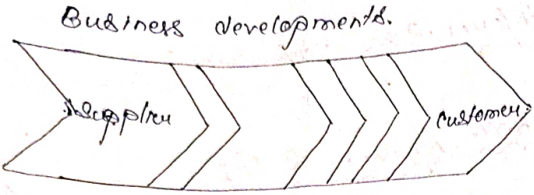
\includegraphics[scale=0.45]{buisdev}
\end{figure}
\begin{itemize}
  \item E-business and e-commerce transformation of business strategies and
    processes.
  \item Agility flexibility and time compression of development manufacturing
    and delivery supply chain cycles.
  \item Re-engineering and cross functional integration of business process 
    using internet technologies.
  \item Competitive advantage, total quality and customer value focus.
\end{itemize}
\textbf{Information technology developments:}
\begin{itemize}
  \item Use of the internet, intranets, extranets and the web as the primary IT
    infrastructure.
  \item Diffusion of technology to inter-networks employees, customer and
    suppliers.
  \item Global and enterprise computing, collaboration and decision support 
    systems.
  \item Integrated cross functional software replaces legacy systems.
\end{itemize}
\textbf{Customer value business value.}
\begin{itemize}
  \item Give customers what they want, when and how they want it at the lowest
    cost.
  \item Inter-enterprise coordination of manufacturing and business process.
  \item Effective distribution and channel partnership.
  \item Responsiveness and accountability to customers.
\end{itemize}%}}}

\subsection{The impact of IT on managers}%{{{
The use of information technology leads to a better management in small and
medium industries. This is very valuable for such industries, because it causes
acquisition of competitive advantage, organizational development, appropriate
reaction against competitors, proper use of the opportunities and threats, and
identification of strengths and weaknesses.%}}}

\subsection{Impact of IT on organization}%{{{
Many companies are re-engineering their organizational structures and roles, as
well as their business processes, as they strive to become agile, customer 
focused, value driven enterprises.

One way to express their phenomenon is illustrated below which outlines several
key dimensions of the new networked organization, compare to the same
dimensions of the new networked organization, compared to the same dimensions
of a traditional organizational model used by many companies. The seven 
dimensions of the networked model demonstrate that IT, particularly e-business 
and e-commerce, appears to make major changes to their organizational
structures and roles.
\begin{itemize}
  \item Organization structures.
  \item Leadership.
  \item People and culture.
  \item Coherence.
  \item Knowledge.
  \item Alliances.
  \item Governance.
\end{itemize}
\begin{figure}[h]
  \centering
  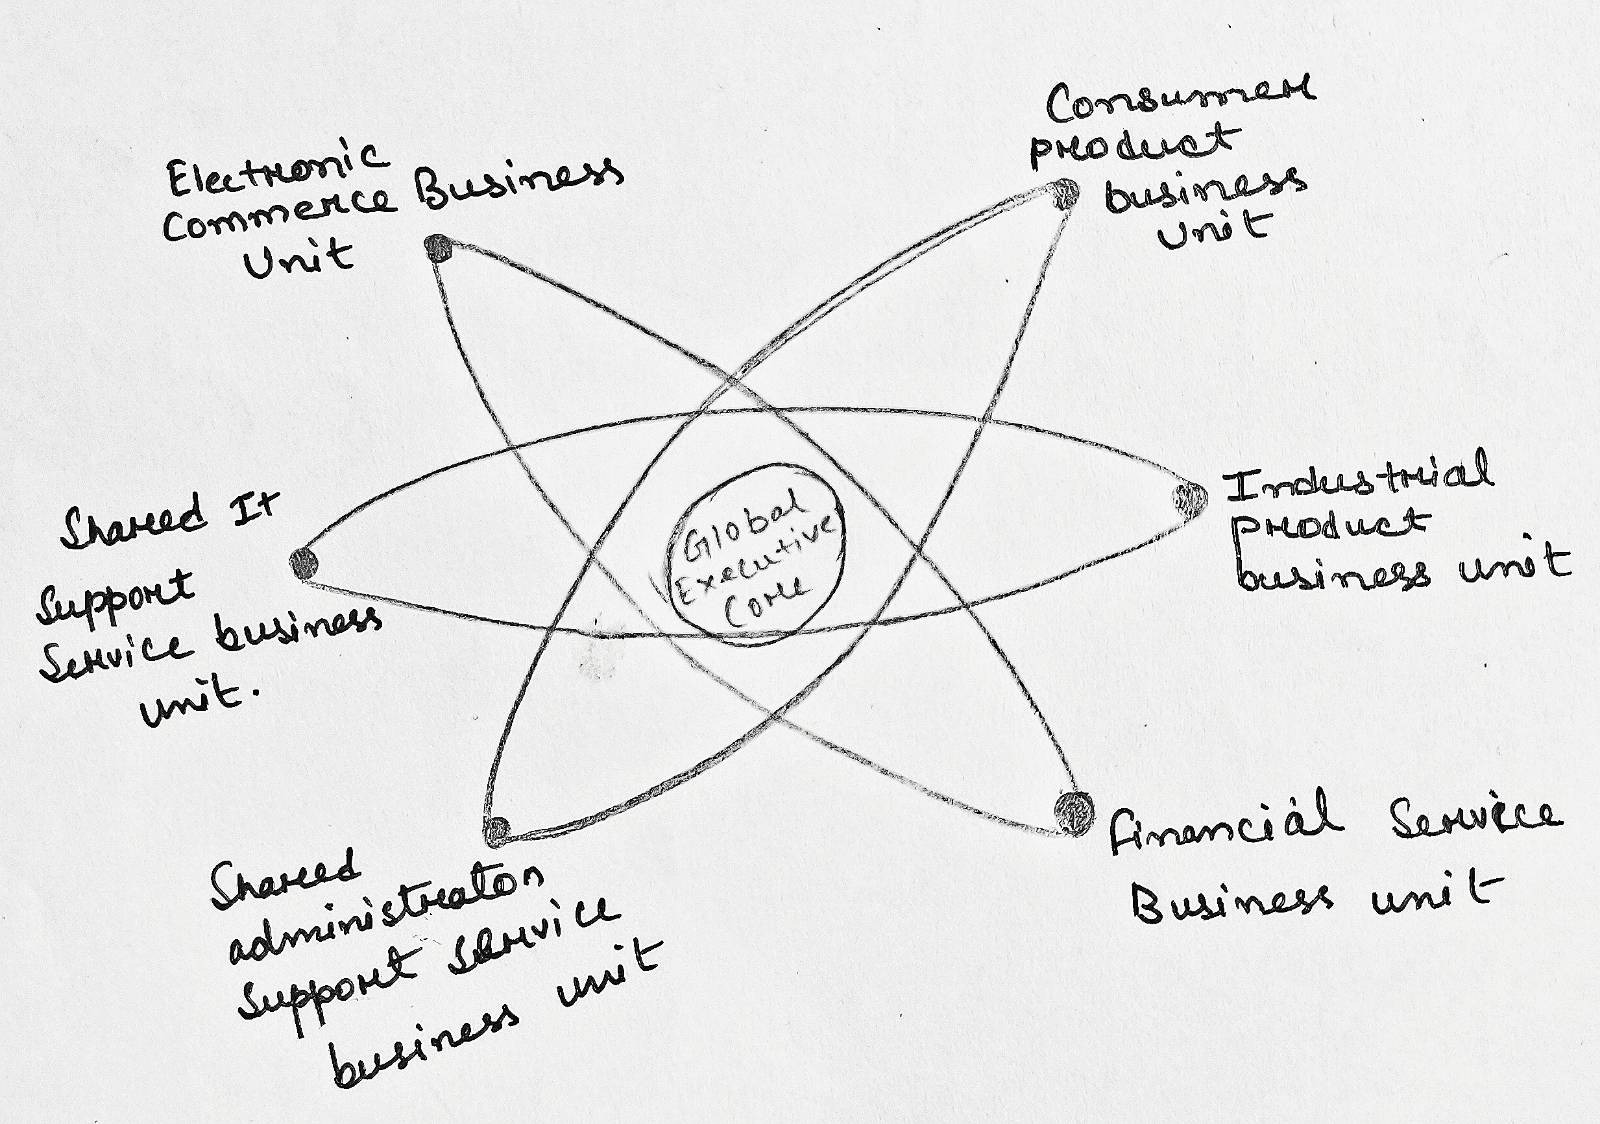
\includegraphics[width=0.48\textwidth]{orgstrucofnetbuis}
  \caption{An example of the organizational structure of a networked business}
\end{figure}%}}}

% Major components of IT management {{{
\begin{figure}[h]
  \centering
  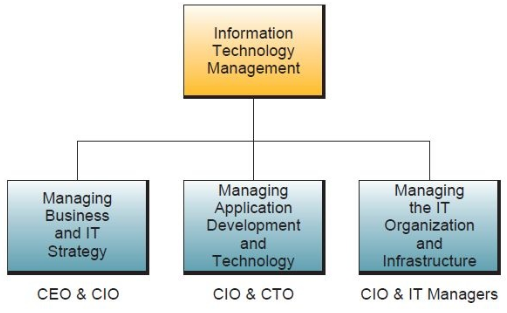
\includegraphics[scale=0.5]{majcompofinfotech}
  \caption{Major components of Information Technology management}
  \label{majcompofinfotech}
\end{figure}%}}}
%}}}

\section{Security and ethical challenges of IT}
\subsection{Security threat}%{{{
A security threat is a malicious act that aims to corrupt or steal data or
disrupt an organization's systems or the entire organization. Information 
Systems are very much prone to security faults which when in hands of cyber
criminals can lead to identity theft, theft of equipment or information, 
information extortion and many more.
\begin{itemize}
  \item Threats are basically system vulnerability that negatively effect
    objects of interests.
  \item Due to lack of maintenance in a commercial environment or untrained
    professionals, software are prone to malware attacks.
\end{itemize}%}}}

\subsection{Ethical issues in IT}%{{{
\begin{itemize}
  \item Misuse of personal information.
  \item Misinformation and deep-fakes.
  \item Lack of oversight and Acceptance of responsibility.
  \item Autonomous technology.
  \item Moral use of data and resources.
  \item Responsible adaptation of disruptive technologies.
\end{itemize}%}}}

\subsection{Security measures}%{{{
\begin{figure}[h]
  \centering
  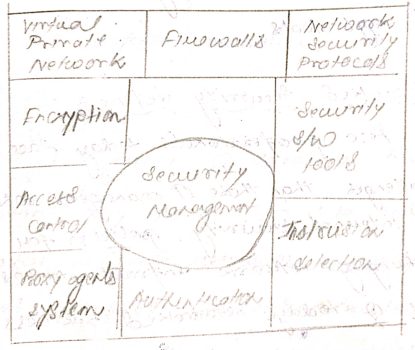
\includegraphics[width=0.48\textwidth]{secmeasure}
  \caption{Importance of security measures that are part of the
  security management of information system}
\end{figure}
\subsubsection{Data Backup}
The most critical type of data security measure. It is done by copying or
archiving data files. As a result, you can retrieve data in case of a data loss
event.

\subsubsection{Firewall}
A firewall is a network security system that monitors and controls incoming
and outgoing network traffic based on predetermined security rules. A
firewall typically establishes a barrier between a trusted network and an
untrusted network, such as the Internet.

\subsubsection{Encryption}
Encryption is the process of encoding information. This process converts the
original representation of the information, known as plain-text, into an
alternative form known as cipher-text. Ideally, only authorized parties can
decipher a cipher-text back to plain-text and access the original information.
Encryption does not itself prevent interference but denies the intelligible
content to a would-be interceptor.

\subsubsection{Security codes}
These are pre-assigned/generated codes that helps authenticate authorized 
personals.%}}}

\section{cybercrime}%{{{
cybercrime is the use of information technology for malicious activity. This 
can range from simply annoying computer users to huge financial loses and even
the loss of human life. With increase in the digitization of modern economy
and society, cybercrime has become a regular occurance.
\subsubsection*{Types of cybercrime:}%{{{
\begin{itemize}
  \item Identity theft.
  \item copyright Infringement.
  \item Click fraud.
  \item Advance fee fraud.
  \item Phising.
  \item Malware.
\end{itemize}%}}}}}}

\section{Digital Signatures}%{{{
It is an electronic, encrypted, stamp of authentication on digital information
such as email, macros, electronic documents, etc. It confirms that the
information originated from the signer and has not been altered.
\begin{figure}[h]
  \centering
  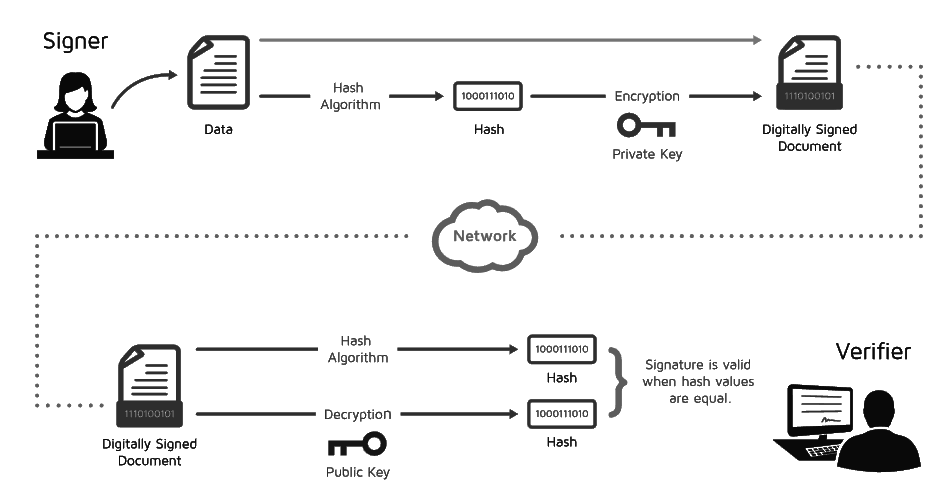
\includegraphics[width=0.5\textwidth]{key}
\end{figure}
\subsection{Advantages of digital signatures}
\begin{enumerate}
  \item Provides better security. Unauthorized person cannot do fraudulence in
    transactions.
  \item Helps you track the status of the documents on which the digital
    signature is applied.
  \item Businesses no longer have to wait for paper documents to be sent by
    courier. Contracts are easily written, completed, and signed by all
    concerned parties in a little amount of time no matter how far the parties
    are geographically.
  \item Signing an electronic document digitally identifies you as the
    signatory and that cannot be later denied.
  \item No one else can forge your digital signature or submit an electronic
    document falsely claiming it was signed by you.
\end{enumerate}

\subsection{Disadvantages of digital signatures}
\begin{enumerate}
  \item Digital signatures, like all technological products, are highly
    dependent on the technology it is based on. In this era of fast
    technological advancements, many of these tech products have a short shelf
    life.
  \item In order to effectively use digital signatures, both senders and
    recipients may have to buy digital certificates at a cost from trusted
    certification authorities.
  \item To work with digital certificates, senders and recipients have to buy 
    verification software at a cost.
  \item In some countries, laws regarding cyber and technology-based issues
    are weak or even non-existent. Trading in such jurisdictions becomes very
    risky for those who use digitally signed electronic documents.
  \item There are many different digital signature standards and most of them
    are incompatible with each other and this complicates the sharing of
    digitally signed documents.
\end{enumerate}%}}}

\section{Privacy issues of information management systems}%{{{
Privacy is an issue that concerns the computer community in connection with
maintaining personal information on individual citizens in computerized record
keeping systems.

Here are some of the most common issues faced by information management
systems:
\subsubsection{Embedding data privacy}
There is a broad lack of information and understanding about embedded
data, where it resides and the financial and reputational risk it posses
to businesses.
\subsubsection{Proliferating devices}
Data privacy becomes harder to handle when you factor in things like the
Internet of Things (IOT), bring-your-own-device IT policies and proliferating
internet-connected tablets, phones and watches.
\subsubsection{Increasing maintenance costs}
Keeping your systems secure and preventing data privacy issues at the
enterprise level can be expensive. But, the costs of a data breach are so
significant, you need to bite the bullet and invest properly.
\subsubsection{Access control is difficult in many industries}
Data privacy breaches are often caused by poorly managed access within an
organization. People and processes matter as much as technology. Humans are
the weakest link in the chain of privacy and security.
\subsubsection{Getting visibility into all of your data}
Using tools to discover and classify your data is essential. This will ensure
you can treat data uniquely and protect your sensitive data from any privacy
issues.
\subsubsection{A bad data culture}
Today, keeping data for its own sake broadens the attack surface for data
theft and increases the risk of breaching many data privacy laws.
Forward-thinking IT teams need to balance the value of collecting, storing and
processing large volumes of data against the pressing requirements for
privacy, security and compliance.
\subsubsection{Ever-increasing scale of data}
With hundreds of systems and millions of data records, we need a solution that
can handle the scale.%}}}

\section{How to prevent computer crime?}%{{{
\begin{center}
  \emph{(Major concerns about computer crime and privacy, and how to
  protect/prevent them.)}
\end{center}
There are different major concerns about computer crime and privacy on the
internet which refers to criminal conduct committed with the aid of a computer
or other electronic equipment connected to the internet.

Individuals or small groups with little technical knowledge and highly
organized worldwide criminal groups with relatively talented developers and 
specialists can engage in cybercrime.

\subsubsection{Stolen credit card information}
The most common cybercrime is when a person's credit card information is
stolen and used unlawfully to acquire or purchase goods or services over the
internet.
\subsubsection{Hacking government databases}
Another type of cybercrime is to tamper with sensitive government information
and data.
\subsubsection{Theft of user accounts}
Many website carrying peoples informations get breached on a regular basis 
nowadays. This results in extortion of user data on the dark web, and is sold 
to the highest bidder.
\subsubsection{Compromised IoT devices}
Most of the IoT devices are kept out of date with regards to their security 
updates, and due to the nature of these devices being connected to the
internet, hackers can get unauthorized access to devices and use those devices
for malicious activity.
\subsubsection{Loss of control and access to content:}
The WannaCry attack, which was allegedly launched by a state sponsored
criminal organization called `the lazurisk' from North-Korea, in 2017,
unleashed ransomware that locked-down thousands of computer mostly from the
NHS(\emph{National Health Security}) network, which are the government
hospitals across UK. Resulting in death of patients, delay in emergency
procedures and all other functions.%}}}

\section{How to protect our-self against cybercrime?}%{{{
\subsubsection{Use strong passwords}
Using a combination of alpha-numaric (abc123), special characters/symbols for a
password creates a hard to crack password. These tho are hard to crack are not
impossible to bypass, it just makes it difficult for anyone to just login to
your account without your permission.

It is also sometimes recommended to use a pass-phrase instead of a password 
due to the hard to guess nature of them.

\subsubsection{Regularly check of security updates}
Keeping softwares upto date is one of the most effective ways to protect a
device agains cyberattacks, these updates usually provide patches to bugs and 
newly discovered exploits and attacker can use to gain access to those devices.

\subsubsection{Keep most personal information off of social media}
This is one of most common yet the most easiest way to find information about
you is from your own social media, with all the digitization of society, every
one shares every single thing about their life, with inturn for someone seeking
to harm you is a goldmine, with these informations, they can do identity theft,
blackmail you, or do find any required informations.

To better protect against such threats, refrain from uploading everything you
do in real life.

\subsubsection{Secure your home network}
Using a local vpn will help you encrypt your unsecure plain \verb+http+ network
traffic into an \verb+https+ connection. This will make any kind of
man-in-the-middle attack impossible.

\subsubsection{Keep up with all major security breaches}
Being aware of all the major databreaches, cyberattacks will help you stay
vigilant and let you know when you need to change your passwords that could
have been breached on certain sites.%}}}

\section{Customer Relationship Management(CRM)}%{{{
Customer relationship management (CRM) is a set of integrated, data-driven
software solutions that help manage, track, and store information related to
your company’s current and potential customers. By keeping this information in
a centralized system, business teams have access to the insights they need, the
moment they need them.

Without the support of an integrated CRM solution, your company may miss growth
opportunities and lose potential revenue because it’s not optimizing operating
processes or making the most of customer relationships and sales leads.

\subsection{Contact and account management}
\begin{figure}[h]
  \centering
  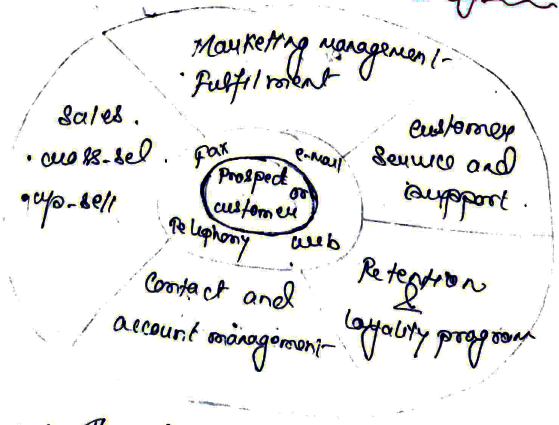
\includegraphics[width=0.47\textwidth]{CRMapplicationcluster}
  \caption{The major application clusters in CRM}
\end{figure}%}}}
 
\section{Procurement Management System}
Procurement management is responsible for overseeing all the processes involved
in acquiring the products, materials, goods and services needed for efficient
business operations. Depending on the business and industry, the terms
`sourcing,' `purchasing' and `procurement' may be used interchangeably to
describe the function of procuring supplies and managing the process, with
sourcing considered more strategic, and purchasing and procurement used to
refer to the actual operational function.

\subsection{Importance of Procurement?}
Without procurement, it would be impossible for most business operations to
function. Procurement management ensures that all items and services are
properly acquired so that projects and processes can proceed efficiently and
successfully.

\subsection{Steps of Procurement process}
\begin{itemize}
  \item [\textbf{Step 1}:] Specifying and planning
  \item [\textbf{Step 2}:] Identifying and selecting suppliers
  \item [\textbf{Step 3}:] Negotiating and contracting
  \item [\textbf{Step 4}:] Placing the purchase order
  \item [\textbf{Step 5}:] Expediting
  \item [\textbf{Step 6}:] Receipt and inspection of purchase
  \item [\textbf{Step 7}:] Invoice clearing and payment
  \item [\textbf{Step 8}:] Maintaining records and relationships
\end{itemize}

\section{ERP}
Enterprise resource planning (ERP) refers to a type of software that organizations use to manage day-to-day business activities such as accounting, procurement, project management, risk management and compliance, and supply chain operations. A complete ERP suite also includes enterprise performance management, software that helps plan, budget, predict, and report on an organization’s financial results.

e.g.:-ERP software for a manufacturing company will typically process the data from and track the status of sales invoicing as well as forecast raw material and HR requirement.
\subsection{Few example of ERP software}
Enterprise Resource Planning or in short ERP refers to the software that most of the businesses, right from the SMEs to enterprises use today for managing day-to-day business operations like accounting, project management, procurement, risk management, supply chain operations, manufacturing, sales and orders, managing customer relationships, human resources, finances, budgeting, reporting, and more. ERP systems are a suite of applications that work for different processes in a business, and stores all the data in a single centralised location, enabling easy transfer of data between the different areas of a business system. ERP software also automates these business activities and reduces time, and human efforts, thereby reducing delicacy of data at the same time.

Some of the amazing business benefits of using ERP software are improved and real-time data insights, low operational costs, enhanced collaboration, better efficiency of processes, elimination of data redundancy, etc.

\subsection{How ERP System works in an organizations like Amazon/Flipkart/Snapdeal?}

ERP systems work via a central database. Users look at dashboards to view real-time data across different business units such as sales, supply chain management, and personnel.
ERP is an integrated system of software applications that allows an organization to manage its business processes using a centralized relational database. It allows a business to see a snapshot of how efficiently its key functions, for example, inventory levels or sales, and personnel are working together.
ERP systems typically contain dashboards connected to a central database that let users look at real-time data across different business units.

\begin{figure}[ht]
  \centering
  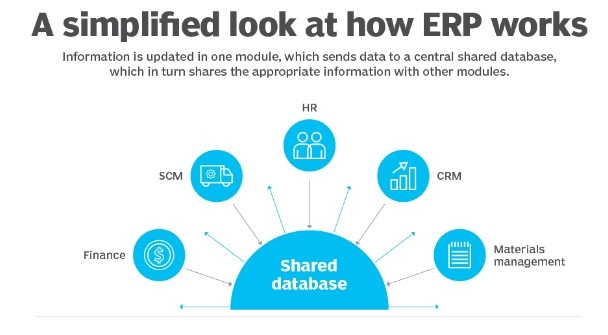
\includegraphics[width=\columnwidth]{howerpworks}
  \caption{A simplified look at how ERP works}
\end{figure}

In an ERP system, information is uploaded in one module and shared to the central database, which shares the information with other modules.

\subsubsection{Purchasing and procurement}
This module is for companies that require all their procurement and purchase activities streamlined, from vendor management to automatically routing approvals of payments and purchase order.

\subsubsection{HR}
This is a centralized digitized HR system that performs tasks from talent management to employee evaluating and tracking personnel hours.

\subsubsection{Finance}
This is a centralized system to track and record sales and operational information and payroll system and that has the ability to perform analysis reporting.

\subsubsection{Customer relationship management}
CRM enables a company to maintain a centralized repository of all the customers which can be accessed and utilized by all the customer oriented departments across the company.

\subsubsection{Business intelligence}
Business intelligence enables companies to view data analytics through dashboards metrics and pre-designed reports.

Amazon/Flipkart basically perform Online sales i.e  also known as e-commerce, the online sales module allows customers to see changes in prices, catalog, inventory and the supply chain, and have those changes reflected in customer-facing messaging. ERP vendors offer e-commerce applications for all sales channels, whether B2B, B2C or C2C. Ideally, this module allows us to manage both consumer and wholesale channels on a single platform. Online sales ERP applications can also let retail or wholesale partners update product information on their end.

\vskip10pt
\begin{table}[ht]
  \resizebox{\columnwidth}{!}{
    \begin{tabular}{|lcr|}
    \toprule
      & Production planning & \\
      &  & \\
      &  & \\
      Sales Distribution & Customer/Employee & Integrated Logistics\\
      &  & \\
      &  & \\
      Order Management & HR & Accountancy and finances\\
    \bottomrule
    \end{tabular}
  }
\end{table}
\begin{figure}[h]
  \caption{Major application components of an ERP system}
\end{figure}

\section{Benefits and challenges of ERP}
\subsection{Quality and Efficiency}
ERP creates a framework for integrating and improving a companies internal business processes that results in significant improvements in the quality and efficiency of customer service production and distribution.

\subsection{Decision Support}
ERP provides vital cross functional information an business performance quickly to managers to significantly improve their ability to make better decisions in timely manner across the entire business enterprise.

\subsection{Enterprise agility}
Implementing ERP system breaks down many former departmental and functional walls of business process is and information resources. This result in most flexible organisational structures , managerial responsibilities and work roles and therefore a more agile and adaptive organisation and work force that can more easily capitalise or new business opportunities.

\subsection{Cost of ERP}
\resizebox{\columnwidth}{!}{
\begin{tabular}{ccc}
  & Hardware & \\
  & 12\% & \\
  Re-engineering & & Software \\
  43\% & & 15\%\\
  & & \\
  Data & & Training and\\
  Conversation & & chair management\\
  15\% & & 15\%\\
\end{tabular}}
\vskip10pt
An ERP implementation is like the corporate equivalent of a brain transplant. We pulled the plug on every company application and moved to people soft software. The risk was certainly disruption of business because if we do not do ERP properly we can kill our company guaranteed.


\section{Supply chain management (SCM)}
Starting an e-business takes ideas capital and technical user. Operating one, however, takes SCM skills. A successful SCM strategy is based on accurate order processing just in time inventory management and timely order fulfilment. SCM’s increasing importance illustrates how a tool that was a theoretical process ten years ago is now a hot competitive weapon. That’s why many companies today are making SCM a top strategic objective and major e-business application development initiative. Fundamentally SCM helps a company get the right products to the right place at the right time in proper quantity and an acceptable cost.

The goal of SCM is a cross functional enterprise system that uses it to helps support and manages the links between same of a compares key business process and low cost network of business relationships or supply chain to get a company’s products from concept to market.

\begin{figure}[ht]
  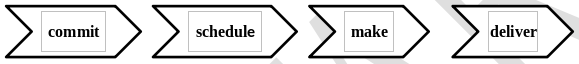
\includegraphics[width=\columnwidth]{scmlc}
  \caption{Supply chain life cycle}
\end{figure}

\section{SCM functional process}
\begin{figure}[ht]
  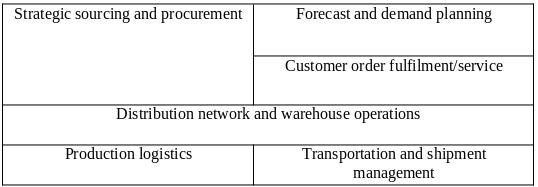
\includegraphics[width=\columnwidth]{scmfuncproc}
\end{figure}


\section{Internet}
\begin{figure}[ht]
  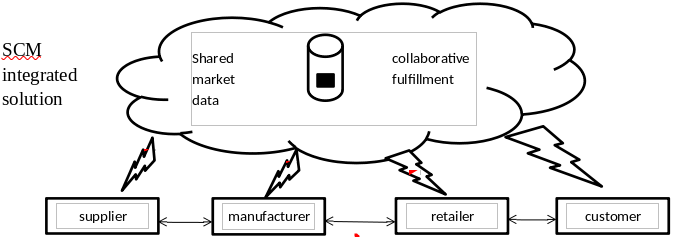
\includegraphics[width=\columnwidth]{scminter}
  \caption{Supply chain management}
\end{figure}

\end{document}
